\documentclass[12pt]{report}

% Packages
\usepackage{acronym}
\usepackage{amsmath}
\usepackage{amsthm}
\usepackage{amsfonts}
\usepackage{epigraph}
\usepackage{geometry}
\usepackage{graphicx}
%\usepackage{mdframed}
\usepackage{titlesec}
\usepackage{caption}
\usepackage{listings}
\usepackage{xcolor}
\usepackage{siunitx}
\usepackage{enumitem}
\usepackage{pdfpages}
\usepackage[utf8]{inputenc}
\usepackage{fancyhdr}
\usepackage{transparent}
\usepackage[hidelinks, colorlinks=true, linkcolor=blue, urlcolor=blue, citecolor=blue]{hyperref}
\usepackage[backend=biber, style=ieee]{biblatex}
%\addbibresource{cdt_app.bib}

% Acronym set-up
% Command to insert acronyms with a temporary color change
\newcommand{\myAcro}[1]{{\hypersetup{linkcolor=black}\acl{#1}}} % For acronym list (full form)
\newcommand{\myAcroLink}[1]{{\hypersetup{linkcolor=black}\acs{#1}}}

% Document geometry setup
\geometry{
    a4paper,
    margin=2cm,
    top=1cm,    % Adjust top margin
    bottom=1cm,  % Adjust bottom margin
    headheight=14.5pt,
    includeheadfoot
}

\pagestyle{fancy} % Use fancy style for all pages
\fancyhf{} % Clear all header and footer fields

% Header
\fancyhead[L]{{\transparent{0.5}Chapter \udlchap{} Questions}} % Left header
\fancyhead[R]{{\transparent{0.5}wp289}} % Right header

% Footer
\fancyfoot[L]{\transparent{0.5}Understanding Deep Learning} % Left footer
\fancyfoot[R]{\transparent{0.5}\thepage} % Right footer

% Define line thickness
\renewcommand{\headrulewidth}{0.4pt}
\renewcommand{\footrulewidth}{0.4pt}

% Redefining plain page style if needed
\fancypagestyle{plain}{ % Applies to chapter beginnings and similar
  \fancyhf{} % clear all header and footer fields for plain style
  \renewcommand{\headrulewidth}{0.4pt}
  \renewcommand{\footrulewidth}{0.4pt}
  \fancyhead[L]{{\transparent{0.5}Chapter \udlchap{}Questions}}
  \fancyhead[R]{{\transparent{0.5}wp289}}
  \fancyfoot[L]{\transparent{0.5}Understanding Deep Learning}
  \fancyfoot[R]{\transparent{0.5}\thepage}
}

% Customise Chapter Headings
\titleformat{\chapter}
    {\normalfont\LARGE\bfseries}
    {\thechapter.}
    {1em}
    {}
\titlespacing*{\chapter}{0pt}{-20pt}{\baselineskip}

% Customise section spacing
\titlespacing*{\section}{0pt}{\baselineskip}{0.5\baselineskip}

% Adjusting space around figures
\setlength{\floatsep}{5pt}
\setlength{\textfloatsep}{5pt}

% Adjusting caption spacing
\captionsetup{aboveskip=5pt, belowskip=5pt}

% Format paragraphs
\setlength{\parindent}{0pt}
\setlength{\parskip}{1em}  % Adjust the value as needed

% Adjust list spacing
%\setlist[enumerate]{before=\vspace{0.5em}, after=\vspace{0.5em}}
\setlist[enumerate]{before=\vspace{-0.5\baselineskip}, after=\vspace{-0.5\baselineskip}}

% Customise question boxes
\usepackage[framemethod=TikZ]{mdframed}
\mdfsetup{
    backgroundcolor=gray!20,
    innertopmargin=10pt,
    innerbottommargin=10pt,
    skipbelow=0pt 
}

\def\udlchap{8}
\renewcommand{\thesubsection}{Problem \udlchap.\arabic{subsection}}

%%%%%%%%%%%%%%%%%%%%%%%%%%%%%%%%%%%%%%%%%%%%%%%%%%%%%%%%%

\begin{document}

\section*{Chapter 8: Measuring performance}

\subsection{}
\begin{mdframed}
    Will the multiclass cross-entropy training loss in figure 8.2 ever reach zero? Explain your reasoning.
\end{mdframed}

Under practical conditions, it is unlikely that the multiclass cross-entropy training loss in figure 8.2 will ever reach zero. As the softmax function is commonly used in the output layer for multiclass classification problems to convert the raw class scores (logits) into probabilities. Due to the exponential function involved in softmax, the predicted probabilities for incorrect classes are unlikely to be exactly zero, even for a very confident model.

\subsection{}
\begin{mdframed}
    What values should we choose for the three weights and biases in the first layer of the model in figure 8.4a so that the hidden unit's responses are as depicted in figures 8.4b-d?
\end{mdframed}

For 8.4b, $\theta_{10} = 0, \text{and} \theta_{11} = 1$, for 8.4c, $\theta_{20} = -0.3, \text{and} \theta_{21} = 1$, and for 8.4d, $\theta_{30} = -0.7$ and $\theta_{31} = 1$.

\subsection{}
\begin{mdframed}
    Given a training set of $I$ input and output pairs $\{x_{i}, y_{i}\}$, show how the parameters \\$\{\beta, \omega_{1},\omega_{2},\omega_{3},\}$ for the model in figure 8.4a using the least squares loss function can be found in closed form.
\end{mdframed}

The key is that the first part of the network is now deterministic; we can compute the activations at the three hidden units for any input. Denoting these by h1, h2 and h3, we now have a linear regression problem:

\begin{equation*}
    y_{i} = \beta + \omega_{1}h_{1i} + \omega_{2}h_{2i} + \omega_{3}h_{3i}
\end{equation*}

where $i$ indexes the training data.

\subsection{}
\begin{mdframed}
    Consider the curve in figure 8.10b at the point where we train a model with a hidden layer of size 200, which would have 50,410 parameters. What do you predict will happen to the training and test performance if we increase the number of training examples from 10,000 to 50,410?
\end{mdframed}

Increasing the number of training examples from 10,000 to 50,410 (increasing training dataset size) would traditionally reduce the variance and therefore improve the generalization performance of the model. This is because the model would have more data to learn from, which would help it to generalize better to unseen data. Therefore, we would expect the test performance to improve.

\subsection{}
\begin{mdframed}
    Consider the case where the model capacity exceeds the number of training data points, and the model is flexible enough to reduce the training loss to zero. What are the implications of this for fitting a heteroscedastic model? Propose a method to resolve any problems that you identify
\end{mdframed}

Heteroscedasticity refers to the condition where the variance of the errors differs across the range of values of an independent variable. The most immediate implication would be that the model overfits to the training data and therefore generalizes poorly to unseen data. To resolve this, we could introduce a regularization term to the loss function to prevent the model from overfitting to the training data or use cross-validation techniques to tune model hyperparameters and select the model complexity that generalizes best to unseen data.

\subsection{}
\begin{mdframed}
    Show that two random points drawn from a 1000-dimensional standard Gaussian distribution are orthogonal relative to the origin with high probability.
\end{mdframed}

For two vectors to be orthogonal, their dot product must be zero. The dot product of two random samples $X$ and $Y$ from a 1000-dimensional standard Gaussian distribution is given by:

\begin{equation*}
    x \cdot y = \sum_{i=1}^{1000} X_{i}Y_{i}
\end{equation*}

Since $X_{i}$ and $Y_{i}$ are independent and identically distributed (i.i.d) with mean 0 and variance of 1, the expected value of $X_{i}Y_{i}$ is also zero and $\text{Var}(X_{i}Y_{i}) = 1$. By the Central Limit Theorem (CLT), as the dimensionality grows, the distribution of the sum (normalized by its standard deviation) will approach a standard normal distribution.

The variance of the sum is the sum of the variances (since the variables are independent):

\begin{equation*}
    \text{Var}(x \cdot y) = \sum_{i=1}^{1000} \text{Var}(X_{i}Y_{i}) = 1000
\end{equation*}

The standard deviation of $X\cdot Y$ is therefore $\sqrt{1000}$. Therefore, as the dimensionality increases, the normalized dot product $(X\cdot Y) / \sqrt{1000}$  will, with high probability, fall within a few standard deviations from 0.

\subsection{}
\begin{mdframed}
    The volume of a hypersphere with radius $r$ in$D$ dimensions is:

    \begin{equation*}
        \text{Vol}[r] = \frac{r^{D}\pi^{D/2}}{\Gamma(D/2 + 1)}
    \end{equation*}

    where $\Gamma{\bullet}$ is the gamma function. Show using Stirling's formula that the volume of a hypersphere of diameter one ($r=0.5$) becomes zero as the dimension increases.
\end{mdframed}

Stirling's formula approximates the gamma function for large $x$ as:

\begin{equation*}
    \Gamma(x) \approx \sqrt{2\pi}x^{x-0.5}e^{-x}
\end{equation*}

Substituting this into the volume formula:

\begin{align*}
    \text{Vol}[0.5] & \approx \frac{(0.5)^{D}\pi^{D/2}}{\sqrt{2\pi}(D/2 + 1)^{D/2}e^{-D/2}}                                   \\
                    & \approx \pi^{\frac{D}{2}-\frac{1}{2}}(0.5\sqrt{2})^{D}(D+2)^{-\frac{D}{2}-\frac{1}{2}}e^{\frac{D}{2}+1}
\end{align*}

The key factor here is the exponential decay caused by the $(0.5\sqrt{2})^{D}$ term. As $D$ increases, this term diminishes much faster than the other components can grow, leading to the overall volume approaching zero.

\subsection{}
\begin{mdframed}
    Consider a hypersphere of radius r = 1. Find an expression for the proportion of the total volume that lies in the outermost $1\%$ of the distance from the center (i.e., in the outermost shell of thickness 0.01). Show that this becomes one as the dimension increases.
\end{mdframed}

Volume of hypersphere of radius $r=1$ is given by:

\begin{equation*}
    \text{Vol}[1] = \frac{\pi^{D/2}}{\Gamma(D/2 + 1)}
\end{equation*}

Volume of hypersphere with radius $r=0.99$ is given by:

\begin{equation*}
    \text{Vol}[0.99] = \frac{(0.99)^{D}\pi^{D/2}}{\Gamma(D/2 + 1)}
\end{equation*}

The proportion $p$ in the last one percent is hence:

\begin{equation*}
    p = \frac{\text{Vol}[1] - \text{Vol}[0.99]}{\text{Vol}[1]} = 1 - 0.99^{D}
\end{equation*}

Which tends to one as $D \rightarrow \infty$.

\subsection{}
\begin{mdframed}
    Figure 8.13c shows the distribution of distances of samples of a standard normal distribution as the dimension increases. Empirically verify this finding by sampling from the standard normal distributions in 25, 100, and 500 dimensions and plotting a histogram of the distances from the center. What closed-form probability distribution describes these distances?
\end{mdframed}

\begin{figure}[h]
    \centering
    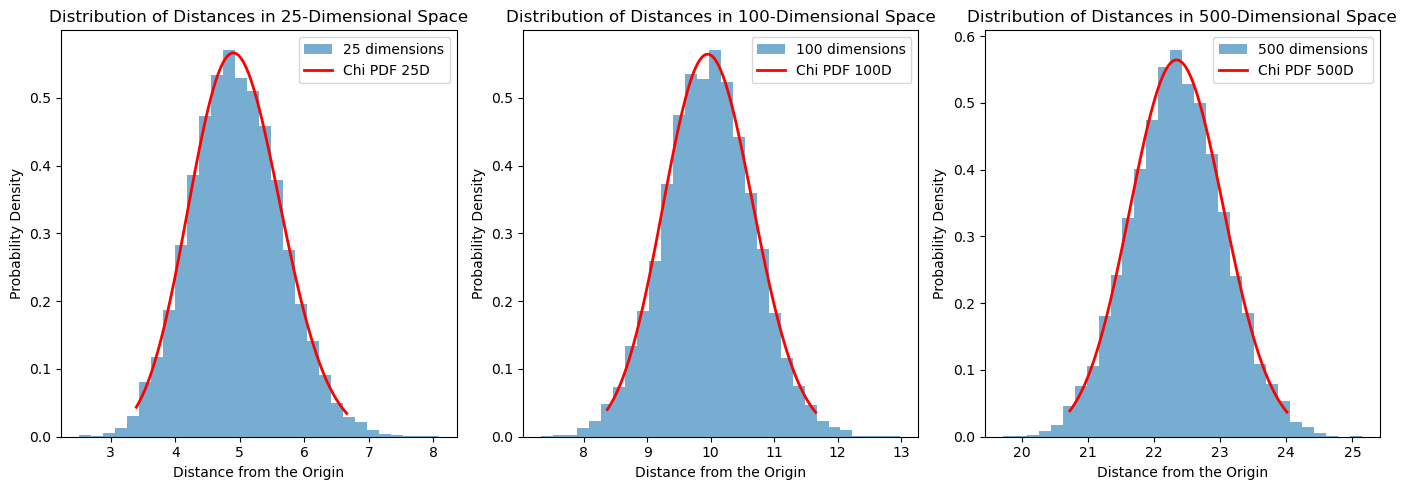
\includegraphics[width=\textwidth]{chap8.png}
    \caption{Distribution of distances of samples of a standard normal distribution as the dimension increases.}
    \label{fig:8_13c}
\end{figure}

The distances appear to follow a normal distribution more closely as the dimensionality increases, this is a reflection of the distances concentrating around their mean due to the dimensions' contribution to the sum of squares.

\end{document}